\setchapterimage[6cm]{chapter/oblast_of_Russia/Flag_maps_of_the_subjects_of_Russia.png}
\chapter{Regions of Russia}
\label{ch:oblast-of-Russia}

\footnotetext{Background image: map of the subjects of the Russian Federation with flags printed on them. Author: \href{https://commons.wikimedia.org/wiki/User:Roman_Poulvas}{Roman Poulvas} (CC BY-SA 4.0).}

This chapter of the book is devoted to the study of the Wikidata regions of Russia. 
Note that the regions of Russia include many lands of different
types: regions, republics, territories and others. It is these diverse regions
that have been studied. A graph of the subjects of Russia bordering
on foreign countries (the graph of neighbors) was built, and a map was drawn
on which the population of individual regions was marked. Assessment
of the degree of occupancy of the Wikidata property <<borders with>> (shares border with) 
it showed that each subject of Russia has these data filled in completely. Two maps were built, on which the border regions and border countries are indicated in color.
The reader will get acquainted with the computer processing of Wikidata and visualization 
information about the regions of Russia.

\label{question:q_subjects_of_Russia_3}
\marginnote{Which entity's flag is in question:
<<The flag of this subject is a rectangular panel with a width-to-length ratio of 2:3, red in color with a two-sided image in the upper corner of the main element of the coat of arms of this subject, which is deployed to the shaft of \href{https://en.wikipedia.org/wiki/Saint_George}{Saint George}. See the answer~\ref{answer:subjects_of_Russia_3} on the page~\pageref{answer:subjects_of_Russia_3}.}

\section{Instances of the object <<Oblast of Russia>>}

To build a list of all regions of Russia, we will need an object 
\wdqName{<<oblast of Russia>>}{835714} and the property \wdProperty{31}{<<instances>>}
(query~\protect\ref{lst:oblast-of-Russia}).

\begin{lstlisting}[ language=SPARQL, numbers=none,
                    caption={List of all regions of Russia. 48 results in 2017 and 46 results in 2021. SPARQL query: \href{https://w.wiki/4D2W}{https://w.wiki/4D2W}},
                    label=lst:oblast-of-Russia,
                    texcl 
                    ]
# List of oblasts of Russia
SELECT ?region ?regionLabel
WHERE
{
  ?region wdt:P31 wd:Q835714. # instance of "oblast of Russia"
  SERVICE wikibase:label { bd:serviceParam wikibase:language "en"}
}
\end{lstlisting}%

In Wikidata, the \wdqName{Leningrad}{2191} and \wdqName{Kaliningrad}{1749} regions have the most properties in Russia and in the world, 43 properties each \autocite{Russia_prowd}.

The regions of Russia with the least number of properties according to ProWD data are: \href{http://www.wikidata.org/entity/Q3129 }{Oryol region} (31 properties), \href{http://www.wikidata.org/entity/Q3178 }{Kursk region} (31 properties), \href{http://www.wikidata.org/entity/Q5851 }{Novosibirsk region} (32 properties).

\section{Subjects of the Russian Federation}

Let's build a list of all the subjects of Russia. To do this, select the following objects in Wikidata: republics, territories, regions, cities of federal significance, autonomous regions and autonomous districts (query~\protect\ref{lst:subjects-of-Russia}).

\marginnote[3.0cm]{Objects used in SPARQL queries:
\begin{itemize}
	\item\wdqName{<<Oblast of Russia>>}{835714};
	\item\wdqName{<<Republic of Russia>>}{41162};
	\item\wdqName{<<Federal city of Russia>>}{183342};
	\item\wdqName{<<Krai of Russia>>}{831740};
	\item\wdqName{<<Autonomus oblast of Russia>>}{309166};
	\item\wdqName{<<Autonomus okrug of Russia>>}{184122};
	\item\wdqName{<<Former administrative-territorial unit>>}{19953632}.
\end{itemize}
Property used \wdProperty{31}{<<instances>>}
}

\begin{lstlisting}[ language=SPARQL, numbers=none,
                    caption={List of all subjects of Russia. 85 results in 2017 and 86 results in 2021. SPARQL query: \href{https://w.wiki/4D2S}{https://w.wiki/4D2S}. In 2021, the federal city of Baikonur was added to the list of subjects on the lease of the complex <<Baikonur>>.},
                    label=lst:subjects-of-Russia,
                    texcl 
                    ]
# List of `instances of` "subjects of Russia" 
SELECT ?subject ?subjectLabel ?typeLabel
WHERE
{  
  VALUES ?type {wd:Q835714   # Oblast of Russia
                wd:Q41162    # Republic of Russia
                wd:Q183342   # Federal city of Russia
                wd:Q831740   # Krai of Russia
                wd:Q309166   # Autonomus oblast of Russia
                wd:Q184122}  # Autonomus okrug of Russia
  ?subject wdt:P31 ?type.  # Selecting the type of object
  SERVICE wikibase:label {bd:serviceParam wikibase:language "en"}
}
\end{lstlisting}%

To build the script ~\protect\ref{lst:subjects-of-Russia} and to verify the results obtained, the following information is needed:
\begin{itemize}
\item According to the Constitution of the Russian Federation, Russia consists of 85 subjects~--- republics, territories, regions, cities of federal significance, autonomous regions, autonomous districts.
  \item This task does not take into account subjects that are not currently part of the Russian Federation (for example, \wdqName{Chita region}{182902}), because they are not instances of objects \wdqName{<<Oblast of Russia>>}{835714}, \wdqName{<<Republic of Russia>>}{41162}, \wdqName{<<Federal city of Russia>>}{183342}, \wdqName{<<Krai of Russia>>}{831740}, \wdqName{<<Autonomus oblast of Russia>>}{309166}, \wdqName{<<Autonomus okrug of Russia>>}{184122}, and belong to the object \wdqName{<<Former administrative-territorial unit>>}{19953632}. (We get 86 objects after executing a SPARQL query, query~\protect\ref{lst:subjects-of-Russia}). 
  \item According to category data <<\href{https://ru.wikipedia.org/wiki/Subjects of the Russian Federation}{Subjects of the Russian Federation}>> of the Russian Wikipedia, there are 85 subjects of the Russian Federation.
  \item According to category data <<\href{https://ru.wikipedia.org/wiki/en:Federal_subjects_of_Russia}{Federal subjects of Russia}>> of the English Wikipedia, there are also 85 subjects of the Russian Federation.
\end{itemize}

\section{Neighboring entities}

Let's construct a graph of neighboring subjects of Russia by the property \wdProperty{47}{shares border with} (query~\protect\ref{lst:sharesBorderWith-oblast-of-Russia}).

\lstset{numbers=left, firstnumber=1, frame=single}
\begin{lstlisting}[ language=SPARQL, 
                    caption={Graph of neighboring subjects of Russia. 467 results in 2017 and 482 results in 2021. SPARQL query: \href{https://goo.su/9ZUj}{Graph of neighboring subjects of Russia}},
                    label=lst:sharesBorderWith-oblast-of-Russia,
                    texcl 
                    ]
# Graph of subjects of Russia "shares border with". 
#defaultView:Graph
SELECT * WHERE {
 {
   SELECT ?subject ?subjectLabel ?rgb ?subjects ?subjectsLabel 
   WHERE {
     SERVICE wikibase:label 
            { bd:serviceParam wikibase:language "en". }
     VALUES ?type {
       wd:Q835714 wd:Q41162 wd:Q183342
       wd:Q831740 wd:Q309166 wd:Q184122
     }
     ?subject wdt:P31 ?type.
   }
 }
 UNION
 { ... }
 UNION
 {
   SELECT ?subject ?subjectLabel ?rgb ?subjects ?subjectsLabel 
   WHERE {
     SERVICE wikibase:label 
            { bd:serviceParam wikibase:language "en". }
     VALUES ?type {
       wd:Q835714 wd:Q41162 wd:Q183342
       wd:Q831740 wd:Q309166 wd:Q184122
     }
     ?subjects wdt:P31 ?type.
     ?oblast wdt:P31 wd:Q835714; wdt:P47 ?subjects.
     
     BIND(IF(?oblast != "", "e87b7b", 
                    IF(?rgb != "", ?rgb, "FFFFFF")) AS ?rgb)
     BIND(IF(?oblast != "", ?oblast, ?subjects) AS ?subject)
     BIND(IF(?oblast != "", ?oblastLabel, 
                    ?subjectsLable) AS ?subjectLable)
   }
 }
}
\end{lstlisting}%

\label{question:q_subjects_of_Russia_1}
\marginnote[-13.0cm]{Name the region of Russia located in the north-west of Russia and formed in \num{1920}. It borders the Leningrad, Vologda, Arkhangelsk and Murmansk regions. It also borders Finland to the west.
Select the flag of this region among the following flags. See the answer \ref{answer:subjects_of_Russia_1} on page~\pageref{answer:subjects_of_Russia_1}.}

\begin{marginfigure}[-10.0cm]
{
	\setlength{\fboxsep}{0pt}%
	\setlength{\fboxrule}{1pt}%
	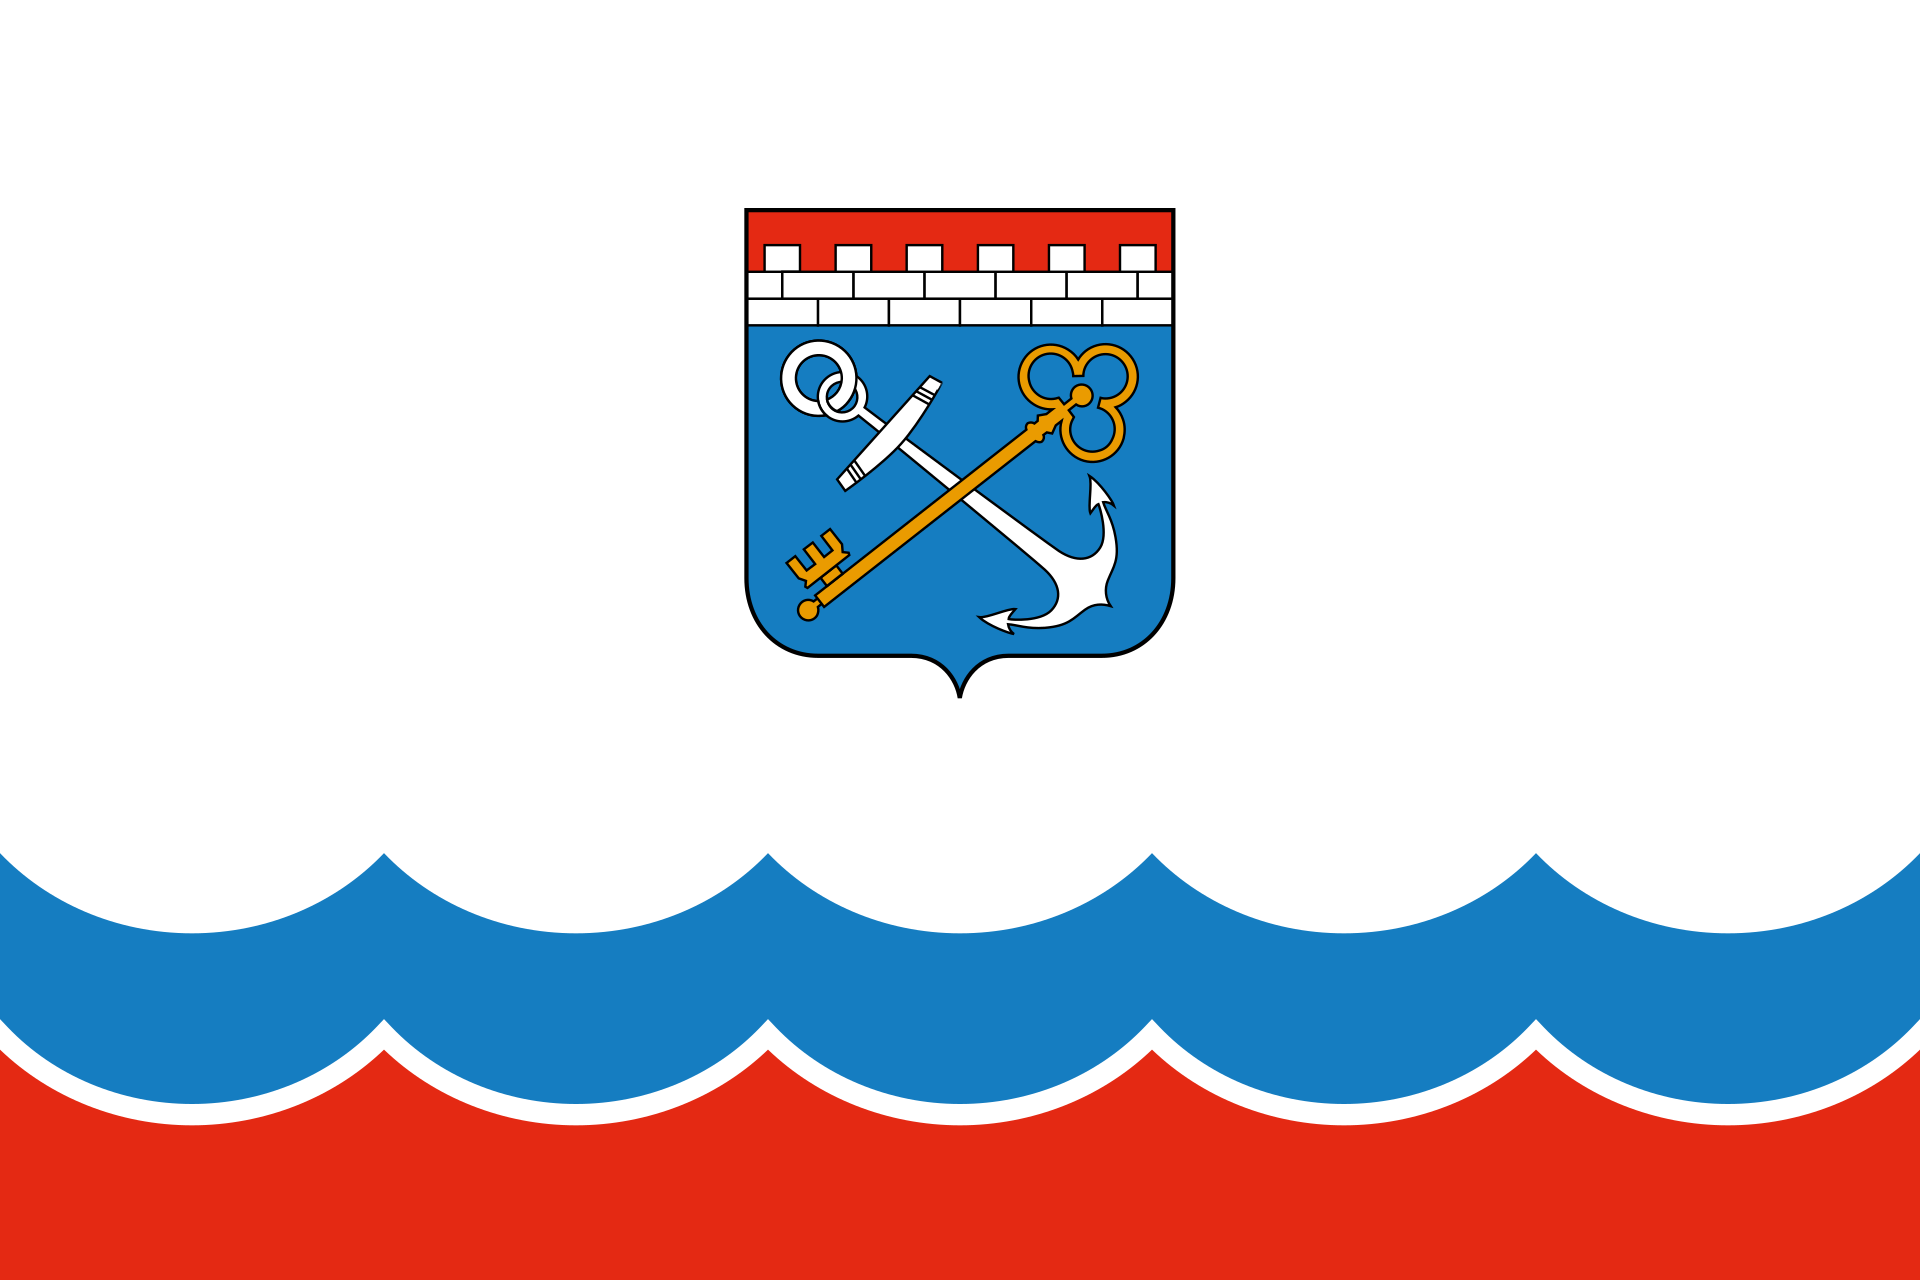
\includegraphics[width=0.8\linewidth]{"chapter/oblast_of_Russia/Flag_of_Leningrad_Oblast.png"}
}
\caption [Flag of the Leningrad region, Russia.]{Flag of the Leningrad region, Russia.}%
\label{fig:Flag_of_Leningrad_Oblast}%
\end{marginfigure}
\begin{marginfigure}[-5.0cm]
{
	\setlength{\fboxsep}{0pt}%
	\setlength{\fboxrule}{1pt}%
	
\includegraphics[width=0.8\linewidth]{"chapter/oblast_of_Russia/Flag_of_Moscow_oblast.png"}
}
\caption [Flag of the Moscow region, Russia.]{Flag of the Moscow region, Russia.}%
\label{fig:Flag_of_Moscow_oblast}%
\end{marginfigure}
\begin{marginfigure}[0.0cm]
{
	\setlength{\fboxsep}{0pt}%
	\setlength{\fboxrule}{1pt}%
	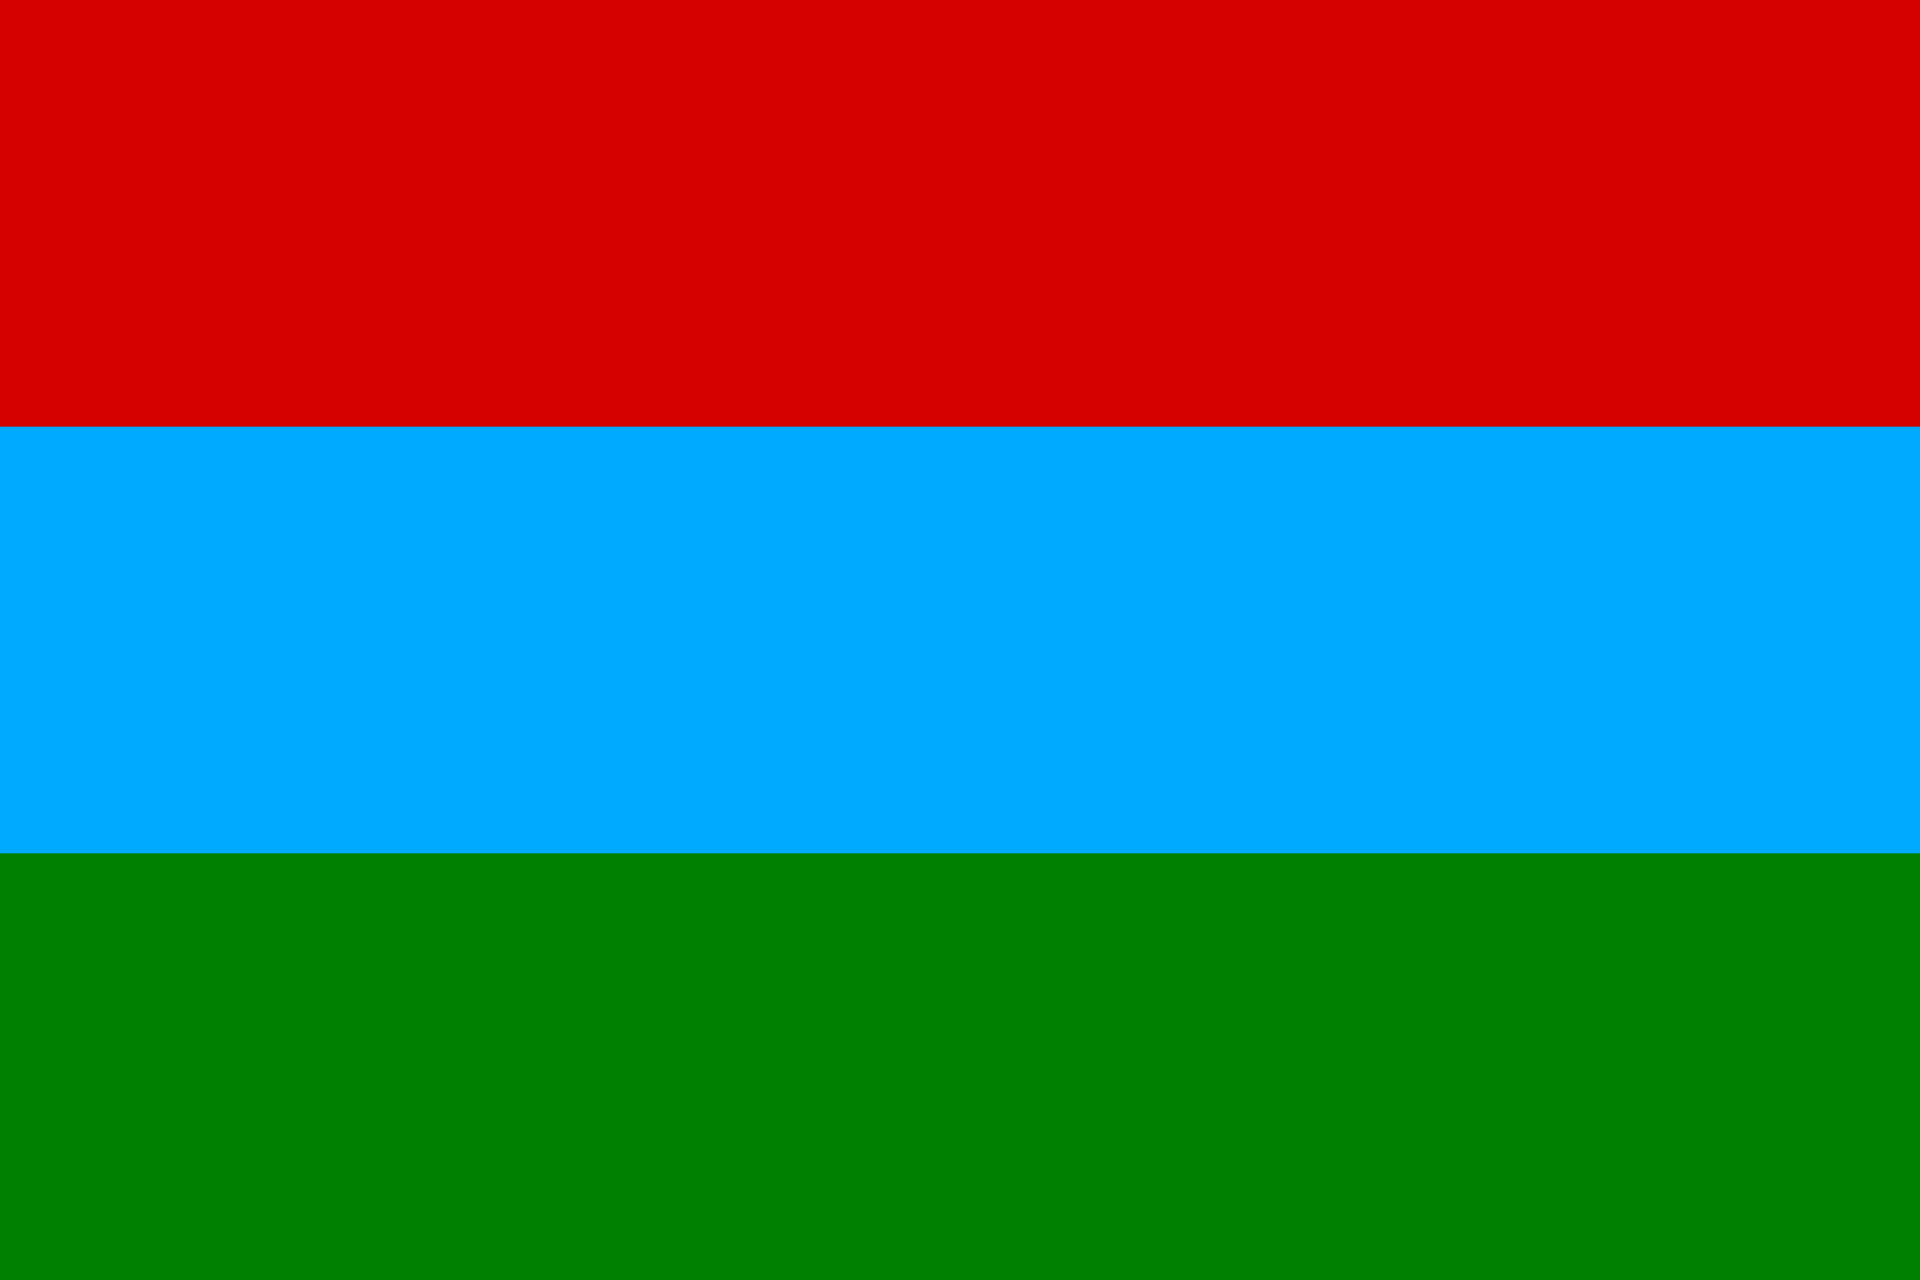
\includegraphics[width=0.8\linewidth]{"chapter/oblast_of_Russia/Flag_of_Karelia.png"}
}
\caption [Flag of Karelia, Russia.]{Flag of Karelia, Russia.}%
\label{fig:Flag_of_Karelia}%
\end{marginfigure}
\begin{marginfigure}[5.0cm]
{
	\setlength{\fboxsep}{0pt}%
	\setlength{\fboxrule}{1pt}%
	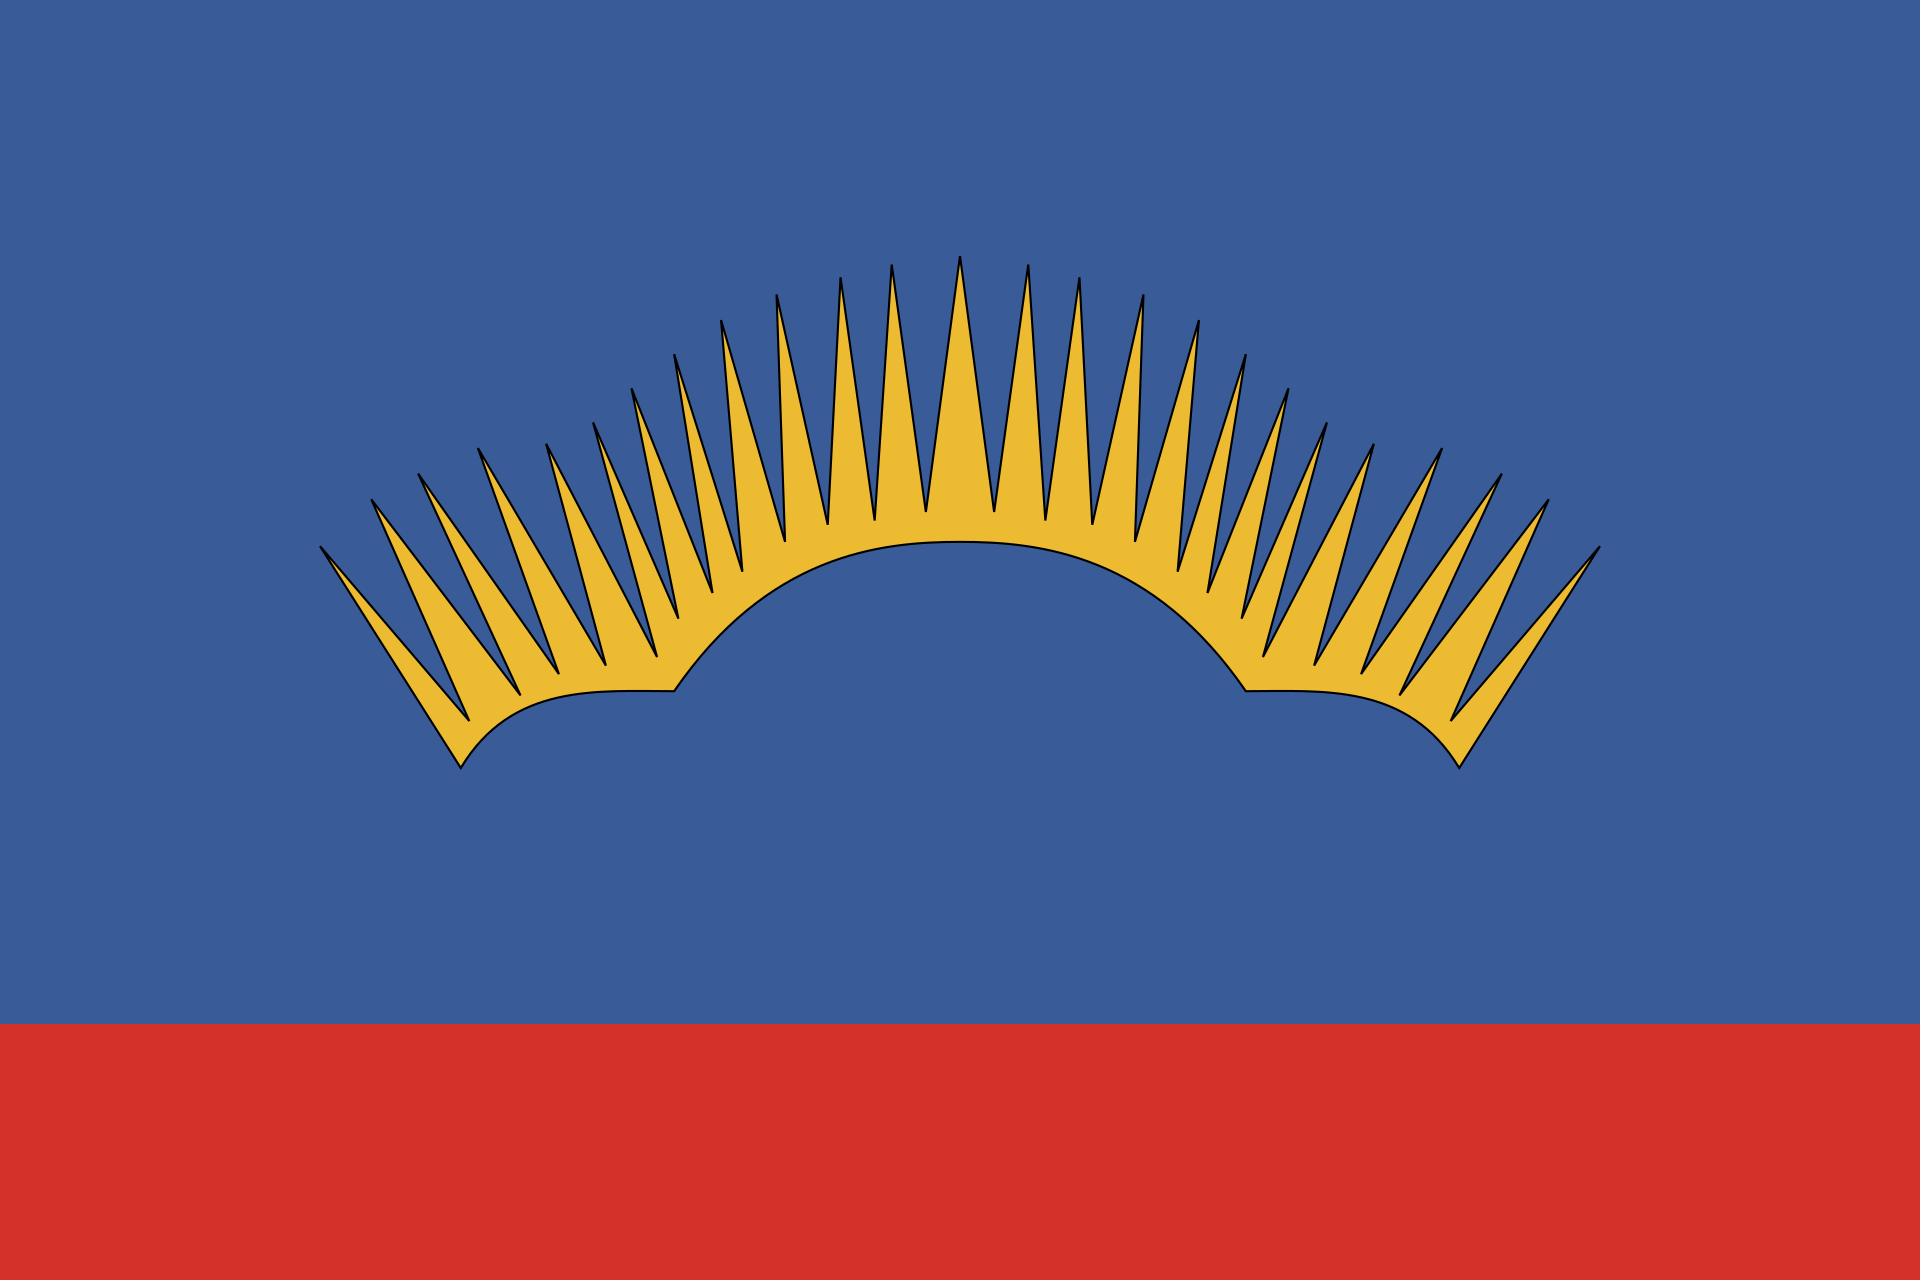
\includegraphics[width=0.8\linewidth]{"chapter/oblast_of_Russia/Flag_of_Murmansk_Oblast.png"}
}
\caption [Flag of the Murmansk region, Russia.]{Flag of the Murmansk region, Russia.}%
\label{fig:Flag_of_Murmansk_Oblast}%
\end{marginfigure}

Using the \textit{BIND} command (lines 31--35) in query~\protect\ref{lst:sharesBorderWith-oblast-of-Russia}, we write the value to a variable, provided that the variable responsible for subjects of a certain type is non-empty. For example, in lines 31--32, a color is written to the variable \textit{?rgb}, provided that \textit{?oblast} is not empty. At the same time, if the variable \textit{?rgb} already contains a value, then we leave it to exclude color mashing.

The number of records received is formed by adding the number of neighboring territories for all subjects of Russia. The result of the script is a graph displaying neighboring subjects. Moreover, different types of subjects have vertices of different colors, for example, the republics are green, and the edges are blue. A part of the graph is shown in Fig.~\ref{fig:sharesBorderWith-oblast-of-Russia-Kaliningrad-fig}.

\begin{figure*}[h]
	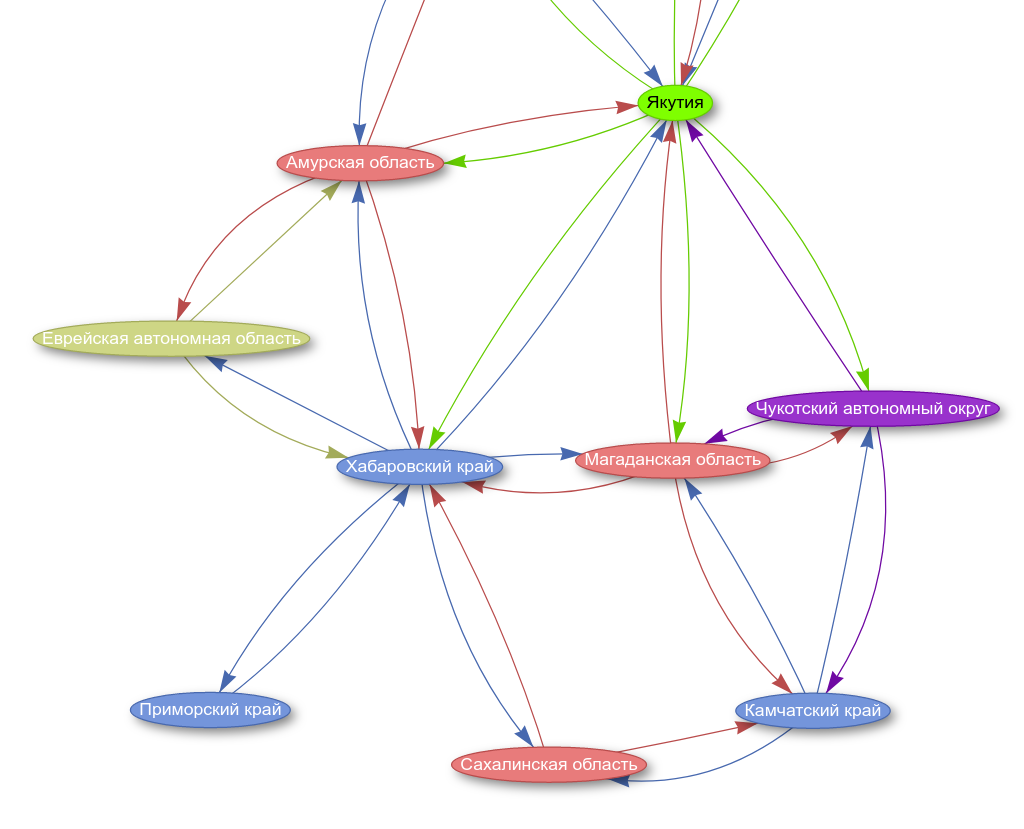
\includegraphics[width=\textwidth]{./chapter/oblast_of_Russia/Graph_Subjects_of_Russia_Siberia_and_the_Far_East_2021.png}
	\caption[Graph of the subjects of Russia. Kaliningrad, 2021.]{Regions of Russia in Siberia and the Far East for 2021. A fragment of the graph of neighboring subjects of Russia, built according to the query~\protect\ref{lst:sharesBorderWith-oblast-of-Russia}.
	Republics~--- green nodes (Yakutia).
	Autonomous Okrugs~--- purple nodes (Chukotka Autonomous Okrug).
	Edges~--- blue nodes (Khabarovsk Krai).
	Areas~--- pink nodes (Amur region).
	Autonomous regions~--- green-colored nodes (Jewish Autonomous Region).}%
      \label{fig:sharesBorderWith-oblast-of-Russia-Kaliningrad-fig}%
\end{figure*}

\newpage
Let's build a map on which the subjects of Russia bordering with foreign countries are indicated in color. The darker color indicates subjects with a larger number of border countries, the lighter~--- with a smaller number of border countries (query~\protect\ref{lst:sharesBorderWith-subjects-of-Russia}).

\lstset{numbers=left, firstnumber=1, frame=single}
\begin{lstlisting}[ language=SPARQL, 
                    caption={Map of the subjects of Russia bordering with foreign countries. 37 results in 2021. SPARQL query: \href{https://w.wiki/4eBf}{Map of Russian regions bordering foreign countries}},
                    label=lst:sharesBorderWith-subjects-of-Russia,
                    texcl 
                    ]
# Map of countries around Russia with the number 
# of neighboring regions of Russia
#defaultView:Map\{"hide":["?shape", "?rgb"], "layer":"?regionLabel"\}
SELECT ?region ?regionLabel ?count ?shape ?rgb
{
  {
    SELECT ?region (COUNT(DISTINCT ?country) AS ?count)
    WHERE {
      VALUES ?type {
        wd:Q835714  # oblasts of Russia - 9 neighbours
        wd:Q41162   # republic of Russia - 4
        wd:Q183342  # federal city of Russia - 0 neighbours
        wd:Q831740  # krai of Russia - 4
        wd:Q309166  # autonomous oblast of Russia - 1
        wd:Q184122   # autonomous okrug of Russia - 1
      }
      ?region wdt:P31 ?type.
  
      # Russian region share border with some territory 
      # of foreign country
      ?region wdt:P47 [ wdt:P17 ?country].
      FILTER (?country != wd:Q159) # foreign country is not Russia
    }
    GROUP BY ?region
    HAVING ((COUNT(?country)) > 0)
  }
  ?region wdt:P3896 ?shape.
  BIND(IF(?count = 3 , "6c2eab", 
            IF(?count = 2 , "9b77bf", 
                IF(?count = 1 , "c6b2db", "f5cbce"))) AS ?rgb)
  SERVICE wikibase:label {bd:serviceParam wikibase:language "en"}  
}
\end{lstlisting}%

The result of the query~\protect\ref{lst:sharesBorderWith-subjects-of-Russia} is shown in the figure~\ref{fig:MapsharesBorderWithsubjectsofRussia}.

\begin{figure*}[h]
	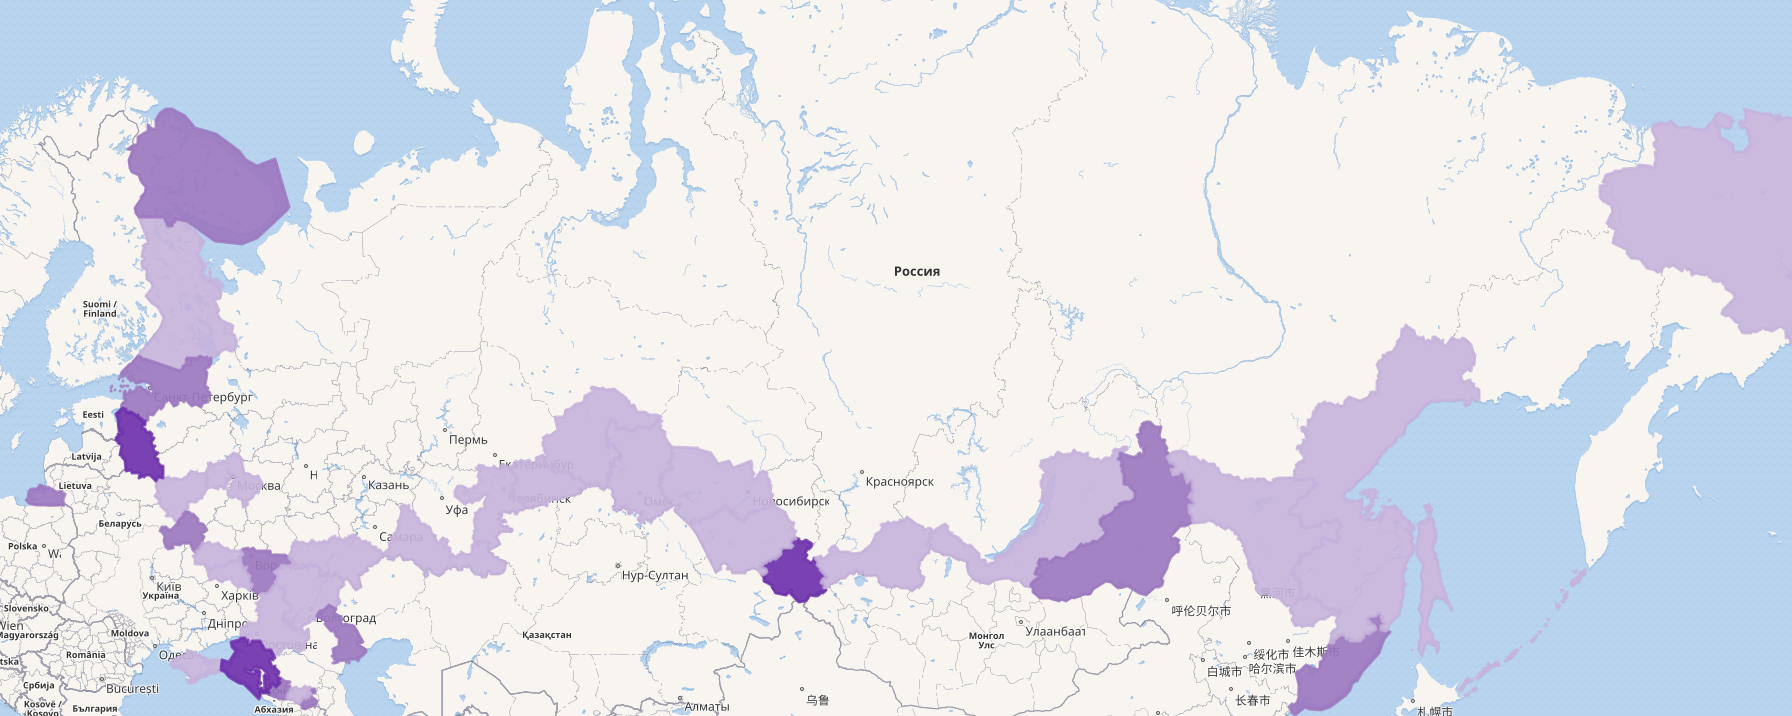
\includegraphics[width=\linewidth]{./chapter/oblast_of_Russia/Maps_of_the_subjects_of_Russia.png}
	\caption[Map of the subjects of Russia bordering on foreign countries, 2021.]{Map of the subjects of Russia bordering on foreign countries, 2021. The map is based on the data received by the request~\protect\ref{lst:sharesBorderWith-subjects-of-Russia}.}%
      \label{fig:MapsharesBorderWithsubjectsofRussia}%
\end{figure*}

Let's build a map on which foreign countries bordering on the subjects of Russia are indicated in color. The darker color indicates the countries with a larger number of border subjects of Russia, the lighter ~--- with a smaller number of border subjects of Russia (query~\protect\ref{lst:Maps_of_the_neighbouring_states_of_Russia}).

\lstset{numbers=left, firstnumber=1, frame=single}
\begin{lstlisting}[ language=SPARQL, 
                    caption={Map of foreign countries bordering the subjects of Russia. 15 results 2021. SPARQL query: \href{https://w.wiki/4eBk}{Map of foreign countries bordering the subjects of Russia}},
                    label=lst:Maps_of_the_neighbouring_states_of_Russia,
                    texcl 
                    ]
# Map of countries around Russia with the number 
# of neighboring regions of Russia
#defaultView:Map\{"hide":["?shape", "?rgb"], "layer": "?countryLabel"\}
SELECT ?country ?countryLabel ?count ?shape ?rgb WHERE {
  {
    SELECT ?country (COUNT(DISTINCT ?region) AS ?count) WHERE {
      VALUES ?type {
        wd:Q835714
        wd:Q41162
        wd:Q183342
        wd:Q831740
        wd:Q309166
        wd:Q184122
      }
      ?region wdt:P31 ?type.
      ?region wdt:P47 [ wdt:P17 ?country].
      FILTER (?country != wd:Q159) # foreign country is not Russia
    }
    GROUP BY ?country
    HAVING ((COUNT(?region)) > 0 )
  }
  ?country wdt:P3896 ?shape.
  BIND(IF(?count > 9 , "4B0082", 
        IF(?count > 5 , "800080", 
         IF(?count > 2 , "8B008B", 
          IF(?count > 1 , "9400D3", 
           IF(?count > 0 , "DA70D6", "f5cbce"))))) AS ?rgb)
  SERVICE wikibase:label {bd:serviceParam wikibase:language "en".}
}
\end{lstlisting}%

The result of the query~\protect\ref{lst:Maps_of_the_neighbouring_states_of_Russia} is shown in the figure~\ref{fig:MapsoftheneighbouringstatesofRussia}.

\begin{figure*}[h]
	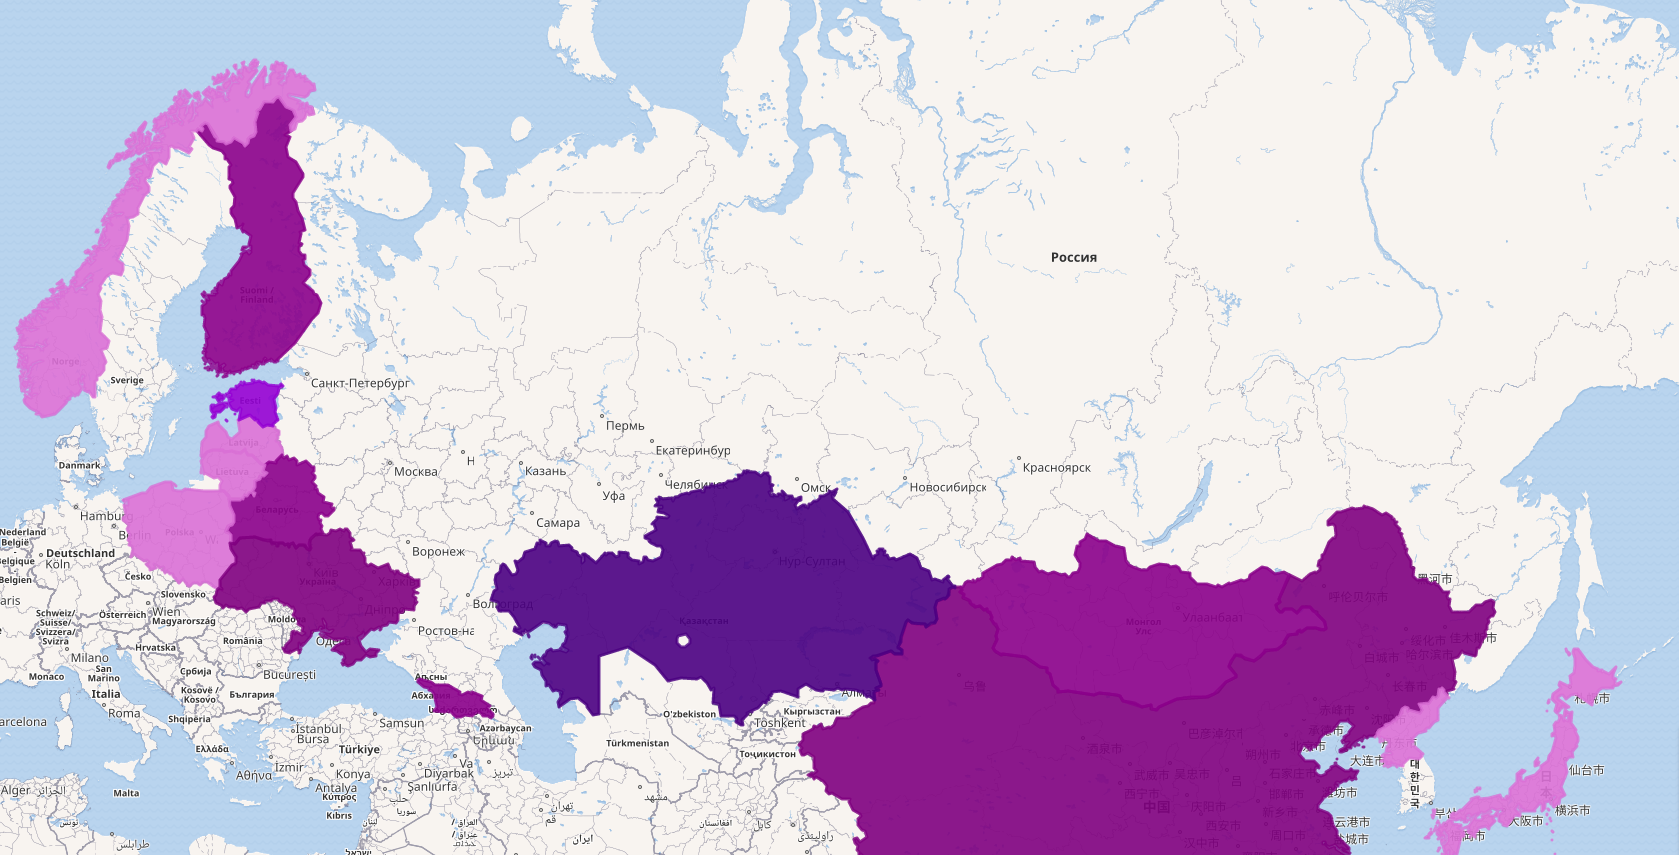
\includegraphics[width=\linewidth]{./chapter/oblast_of_Russia/Maps_of_the_neighbouring_states_of_Russia.png}
	\caption[Map of foreign countries bordering the subjects of Russia, 2021.]{Map of foreign countries bordering the subjects of Russia, 2021. The map is based on the data received by the request~\protect\ref{lst:Maps_of_the_neighbouring_states_of_Russia}.}%
      \label{fig:MapsoftheneighbouringstatesofRussia}%
\end{figure*}

\newpage
\subsection{Completeness of Wikidata}

Let's build a list of subjects of Russia with an empty property \wdProperty{47}{shares border with} (borders with) (query~\protect\ref{lst:sharesBorderWith-empty-oblast-of-Russia}), that is, we will try to find such subjects that do not share border with anyone.

\label{question:q_subjects_of_Russia_2}
\marginnote[4.0cm]{Which of the following subjects are currently part of the Russian Federation, and which are not:
\begin{itemize}
  \item Republic of Adygea;
  \item Kamchatka Krai;
  \item Chita region;
  \item Chukotka Autonomous Okrug.
\end{itemize}
See the answer \ref{answer:subjects_of_Russia_2} on page~\pageref{answer:subjects_of_Russia_2}.
}

\lstset{numbers=left, firstnumber=1, frame=single}
\begin{lstlisting}[ language=SPARQL, 
                    caption={List of subjects of the Russian Federation with an empty property \wdProperty{47}{shares border with}. 0 results in 2017 and 0 results in 2021. SPARQL query: \href{https://w.wiki/4bLL}{https://w.wiki/4bLL}},
                    label=lst:sharesBorderWith-empty-oblast-of-Russia,
                    texcl 
                    ]
# List of `subjects of Russia`~without `shares border with`. 
SELECT 
    ?subject ?subjectLabel 
    ?sharesBorderWith ?sharesBorderWithLabel
WHERE
{
  VALUES ?type {wd:Q835714   # Oblast of Russia
                wd:Q41162    # Republic of Russia
                wd:Q183342   # Federal city of Russia
                wd:Q831740   # Krai of Russia
                wd:Q309166   # Autonomus oblast of Russia
                wd:Q184122}  # Autonomus okrug of Russia
  
  ?subject wdt:P31 ?type.
  
  FILTER EXISTS {?subject wdt:P17 wd:Q159; wdt:P31 ?type}
  
  MINUS { ?subject  wdt:P47 [] } . #Shares border with 
  SERVICE wikibase:label { bd:serviceParam wikibase:language "en"}
}
\end{lstlisting}%

Using the \textit{FILTER} command (line 16), we exclude objects that are not located on the territory of Russia. Then, using \textit{MINUS} (line 20), we select objects whose property \wdProperty{47}{<<shares border with>>} is not filled.

Thus, the \wdProperty{47}{<<shares border with>>} property is filled on Wikidata for all subjects of Russia.

\section{Population of individual subjects of the Russian Federation}

Let's mark the subjects of the Russian Federation on the map, dividing them into six groups by population. Subjects belonging to the same group will be displayed on the map in the same color.

For the query~\protect\ref{lst:map} we need the properties \wdProperty{625}{<<coordinates>>} and \wdProperty{1082}{<<population>>}.

\index{Graph!Map!Map of the population of Russia}

\begin{lstlisting}[ language=SPARQL, numbers=none,
                    caption={Map of the population of Russia. 85 results in 2017 and 86 results in 2021. SPARQL query: \href{https://w.wiki/4bLQ}{https://w.wiki/4bLQ}},
                    label=lst:map,
                    texcl 
                    ]
# Map of population by subjects of Russia
# Version 2021
#defaultView:Map
SELECT DISTINCT ?subject ?subjectLabel ?population ?coord ?layer
{
  {
    { ?subject wdt:P31 wd:Q835714 } UNION  # Oblast of Russia
    { ?subject wdt:P31 wd:Q41162 } UNION  # Republic of Russia
    { ?subject wdt:P31 wd:Q183342 } UNION  # Federal city of Russia
    { ?subject wdt:P31 wd:Q831740 } UNION  # Krai of Russia
    { ?subject wdt:P31 wd:Q309166 } UNION # Autonomus oblast 
                                          #             of Russia
    { ?subject wdt:P31 wd:Q184122 } # Autonomus okrug of Russia
  }   
  ?subject wdt:P625 ?coord; wdt:P1082 ?population.
  
  BIND(
    IF(?population < 500000, "< 500000",
    IF(?population < 1000000, "500000 - 1000000",
    IF(?population < 3000000, "1000000 - 3000000",
    IF(?population < 8000000, "3000000 - 8000000",
    IF(?population < 10000000, "8000000 - 10000000",
    "> 10000000")))))
    AS ?layer).
  
  SERVICE wikibase:label { bd:serviceParam wikibase:language "en"}
}
ORDER BY ?population
\end{lstlisting}%

The result of the script (listing~\protect\ref{lst:map}) is shown in the figure~\ref{fig:SubjectsRussiaMap}.

%\begin{fullwidth}
\begin{figure*}[h]
	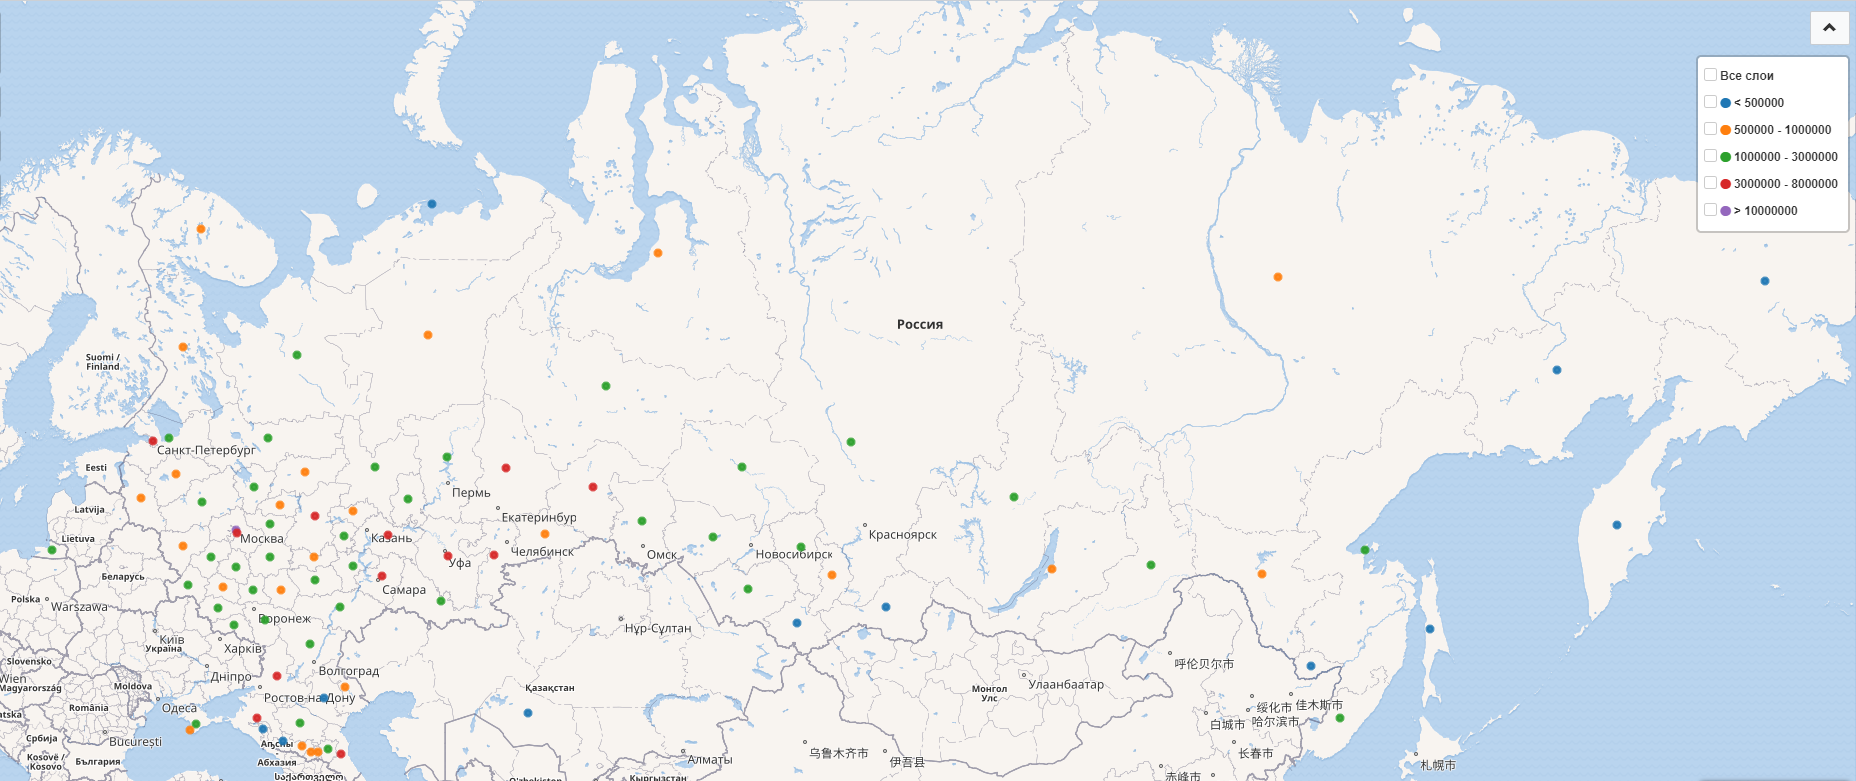
\includegraphics[width=1.0\linewidth]{./chapter/oblast_of_Russia/SubjectsRussia_Map_with_legend_RU.png}
	\caption[Map of the population by subjects of Russia, 2021.]{Population map by subjects of Russia, 2021. The subjects are divided into six groups by population and marked with different colors depending on the group the subject belongs to. The map is based on the data received by the request~\protect\ref{lst:map}.}%
      \label{fig:SubjectsRussiaMap}%
\end{figure*} 
%\end{fullwidth}

